\documentclass[10pt]{exam}
\usepackage[phy]{template-for-exam}
\usepackage{empheq, multicol, pgfplots}
\pgfplotsset{
  compat=1.18,
  width=6cm,
  posgraph/.append style={
    axis y line = left,
    axis x line = center,
    axis line style = ultra thick,
    xlabel={\bf time},
    ylabel={\bf displacement},
    ymin=0,
    ymax=9,
    xmin=0,
    xmax=3,
    xtick=\empty,
    ytick=\empty,
  },
  velgraph/.append style={
    xlabel={\bf time},
    ylabel={\bf velocity},
    ymin=-5,
    ymax=5,
    xmin=0,
    xmax=4,
    ytick=\empty,
    xtick=\empty,
    axis y line = left,
    axis x line = center,
    axis line style = ultra thick,
  },
  numberedplots/.append style={
    xlabel={\bf time (s)},
    width=7cm,
    ytick={-15,...,15},
    xtick={0,...,5},
    axis y line = left,
    axis x line = center,
    grid=major,
    axis line style = ultra thick,
  },
}
%\printanswers
\shadedsolutions

\title{Unit 01 Review}
\author{Rohrbach}
\date{\today}

\newcommand{\printeqs}{
  \begin{center}
    \vspace{-0.5cm}
    \begin{empheq}[box=\fbox]{align*}
     &
     & 
      v &= \frac{d}{t}        &    
      a &= \frac{\Delta v}{t} &
      \Delta v &= v_f - v_i   &
     &
    \end{empheq}
  \end{center}
}


\begin{document}
\maketitle

\ifprintanswers
\else
  \printeqs
\fi

\begin{questions}

  \question Define the following terms

    \begin{parts}
      \part distance
        \begin{solution}[1em]
          total amount traveled by an object (a scalar)
        \end{solution}
      
      \part displacement
        \begin{solution}[1em]
          how far an object is from its starting point (a vector)
        \end{solution}

      \part speed
        \begin{solution}[1em]
          how fast an object travels (a scalar)
        \end{solution}

      \part velocity
        \begin{solution}[1em]
          speed and direction (a vector)
        \end{solution}

      \part acceleration
        \begin{solution}[1em]
          the rate that velocity changes (a vector)
        \end{solution}

    \end{parts}
    \vspace{2em}
    
  \question
    What is the acceleration of a ping-pong ball that is initially traveling at $15$ m/s, and then is returned to the other player with a velocity of $-15$ m/s in $0.2$ s?

    \begin{solution}[\stretch{1}]
      \vspace{-1.5em}
      \begin{align*}
        v_i & = 15~\text{m/s} &
                            a &= \frac{v_f-v_i}{t} \\
        v_f & = 15~\text{m/s} &
                            &= \frac{-15-15}{0.2} \\
        t   & = 0.2~\text{s} &
                            &= -150~\text{m/s}^2 \\
        a   & = \text{?} 
      \end{align*}
      \vspace{-1.5em}
    \end{solution}
  
  \question
    What is the final velocity of an ice cream truck that has an initial velocity of $5$ m/s, and accelerates at $2.1$ m/s$^2$ for $7.3$ s?

    \begin{solution}[\stretch{1}]
      \vspace{-1.5em}
      \begin{align*}
        v_i & = 5~\text{m/s} &
                            a    &= \frac{v_f-v_i}{t} \\
        a & = 2.1~\text{m/s}^2 &
                            2.1  &= \frac{v_f-5}{7.3} \\
        t   & = 7.3~\text{s} &
                           15.33 &= v_f-5 \\
        v_f   & = \text{?} &
                           20.33~\text{m/s} &= v_f 
      \end{align*}
      \vspace{-1.5em}
    \end{solution}

  \question
    How much time will it take an octopus that swims at $23$ m/s to travel $82$ m?
    
    \begin{solution}[\stretch{1}]
      \vspace{-1.5em}
      \begin{align*}
        v &= 23~\text{m/s} &      v &= \frac{d}{t}    \\
        d &= 82~\text{m}^2 &     23 &= \frac{82}{t}   \\
        t &= \text{?}      &    23t &= 82             \\
          &                &      t &= 3.57~\text{s}
      \end{align*}
      \vspace{-1.5em}
    \end{solution}

  \pagebreak
  
  \question
    What does it mean to say that an object is accelerating at \SI{10}{\meter\per\second^2}\,?
    
    \begin{solution}[1.5cm]
      The object's velocity is changing by 10 m/s every second.
    \end{solution}

  \question
    Consider this graph of a motor boat's displacement over time.

    \begin{multicols}{2}
      \begin{parts}
        \part
          The object is moving
    
          \begin{oneparcheckboxes}
            \correctchoice forward
            \choice backward
          \end{oneparcheckboxes}
    
        \part
          The object is
    
          \begin{checkboxes}
            \choice speeding up
            \choice slowing down
            \correctchoice moving at a constant speed
          \end{checkboxes}
    
        \part
          Calculate the velocity.
            \begin{solution}[.75cm]
              \SI{0.75}{\meter\per\second}
            \end{solution}
    
        \part
          Calculate the acceleration.
            \begin{solution}[.75cm]
              \SI{0}{\meter\per\second^2}
            \end{solution}
    
    
      \end{parts}

      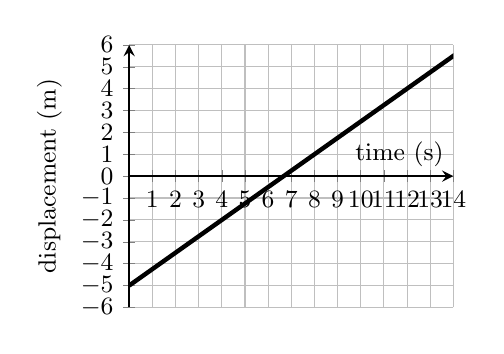
\begin{tikzpicture}
        \begin{axis}[
          axis y line = box,
          axis x line = box,
          axis line style = thick,
          axis x line = center,
          axis y line = left,
          xlabel={\small time (s)},
          ylabel={\small displacement (m)},
          ymin=-6,
          ymax=6,
          xmin=0,
          xmax=14,
          grid=both,
          xtick = {0,...,17},
          ytick = {-7,...,7},
          width=.47\textwidth,
          ticklabel style = {font=\small},
        ]
          \addplot[ultra thick,domain=0:17]{.75*x-5};
        \end{axis}
      \end{tikzpicture}

    \end{multicols}

  \question
    Consider this graph of this train's velocity over time.

    \begin{multicols}{2}
      
      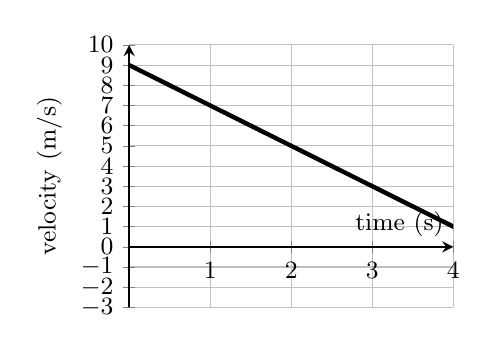
\begin{tikzpicture}
        \begin{axis}[
          axis y line = box,
          axis x line = box,
          axis line style = thick,
          axis x line = center,
          axis y line = left,
          xlabel={\small time (s)},
          ylabel={\small velocity (m/s)},
          ymin=-3,
          ymax=10,
          xmin=0,
          xmax=4,
          grid=both,
          xtick = {0,...,17},
          ytick = {-7,...,10},
          width=.47\textwidth,
          ticklabel style = {font=\small},
        ]
          \addplot[ultra thick,domain=0:17]{-2*x+9};
        \end{axis}
      \end{tikzpicture}
      
      \begin{parts}
        \part
          The object is moving
    
          \begin{oneparcheckboxes}
            \correctchoice forward
            \choice backward
          \end{oneparcheckboxes}
    
        \part
          The object is
    
          \begin{checkboxes}
            \choice speeding up
            \choice slowing down
            \correctchoice moving at a constant speed
          \end{checkboxes}
    
        \part
          Calculate the acceleration.
            \begin{solution}[.75cm]
              \SI{-2}{\meter\per\second^2}
            \end{solution}
    
    
      \end{parts}

    \end{multicols}

  \question
    A bear walks 50 m east in 60 s.  Then, he turns around and walks 50 m west back to his starting point in 120 s.  What is his (a) speed and (b) velocity for the entire trip?

    \begin{solution}
      \begin{multicols}{2}

        \begin{align*}
          \text{distance} &= 50~\text{m} + 50~\text{m} = 100~\text{m} \\
          \text{displacement} &= 50~\text{m} - 50~\text{m} = 0 \\
          \text{total time} &= 60~\text{s} - 120~\text{s} = 180~\text{s} \\ 
          \\
          \text {speed} &= \frac{\text{distance}}{\text{time}} = \frac{100}{180} = 0.56~\text{m/s} \\
          \text {velocity} &= \frac{\text{displacement}}{\text{time}} = \frac{0}{180} = 0~\text{m/s}
        \end{align*}

        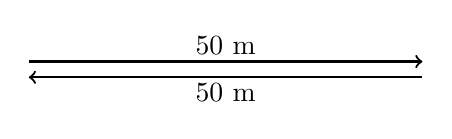
\begin{tikzpicture}
          \draw [thick,->] (0,0) -- (5,0);
          \draw [thick,<-] (0,-.2) -- (5,-.2);
          \node at (2.5,0.2) {50 m};
          \node at (2.5,-0.4) {50 m};
        \end{tikzpicture}

      \end{multicols}
    \end{solution}



  % \pagebreak

  % \question Indicate what each object is doing.

  % \begin{multicols}{3}
  %   \begin{parts}
  %     \small
  %     \part \hfill

  %       \begin{tikzpicture}
  %         \begin{axis}[posgraph,width=5cm]
  %           \addplot[smooth,domain=0.2:2.5]{2*x+1};
  %         \end{axis}
  %       \end{tikzpicture}
        
  %       Object is moving

  %       \begin{oneparcheckboxes}
  %         \correctchoice forward
  %         \choice backward
  %       \end{oneparcheckboxes}
        
  %       Speed is
        
  %       \begin{oneparcheckboxes}
  %         \choice increasing
  %         \choice decreasing
  %         \correctchoice constant
  %       \end{oneparcheckboxes}

  %       \vspace{1em}

  %     \part \hfill

  %       \begin{tikzpicture}
  %         \begin{axis}[velgraph,width=5cm]
  %           \addplot[smooth,domain=0.2:3]{x-4};
  %         \end{axis}
  %       \end{tikzpicture}

  %       Object is moving

  %       \begin{oneparcheckboxes}
  %         \choice forward
  %         \correctchoice backward
  %       \end{oneparcheckboxes}
        
  %       Speed is
        
  %       \begin{oneparcheckboxes}
  %         \choice increasing
  %         \correctchoice decreasing
  %         \choice constant
  %       \end{oneparcheckboxes}

  %       \vspace{1em}

  %     \part \hfill

  %       \begin{tikzpicture}
  %         \begin{axis}[posgraph,width=5cm]
  %           \addplot[smooth,domain=0.2:2.5]{-x^2+8};
  %         \end{axis}
  %       \end{tikzpicture}

  %       Object is moving

  %       \begin{oneparcheckboxes}
  %         \choice forward
  %         \correctchoice backward
  %       \end{oneparcheckboxes}
        
  %       Speed is
        
  %       \begin{oneparcheckboxes}
  %         \correctchoice increasing
  %         \choice decreasing
  %         \choice constant
  %       \end{oneparcheckboxes}

  %     \part \hfill

  %       \begin{tikzpicture}
  %         \begin{axis}[velgraph,width=5cm]
  %           \addplot[smooth,domain=0.2:3]{x+1};
  %         \end{axis}
  %       \end{tikzpicture}

  %       Object is moving

  %       \begin{oneparcheckboxes}
  %         \correctchoice forward
  %         \choice backward
  %       \end{oneparcheckboxes}
        
  %       Speed is
        
  %       \begin{oneparcheckboxes}
  %         \correctchoice increasing
  %         \choice decreasing
  %         \choice constant
  %       \end{oneparcheckboxes}

  %     \part \hfill

  %       \begin{tikzpicture}
  %         \begin{axis}[posgraph,width=5cm]
  %           \addplot[smooth,domain=0.2:2.5]{3^(-x+2.1)+1};
  %         \end{axis}
  %       \end{tikzpicture}

  %       Object is moving

  %       \begin{oneparcheckboxes}
  %         \choice forward
  %         \correctchoice backward
  %       \end{oneparcheckboxes}
        
  %       Speed is
        
  %       \begin{oneparcheckboxes}
  %         \choice increasing
  %         \correctchoice decreasing
  %         \choice constant
  %       \end{oneparcheckboxes}

  %     \part \hfill

  %       \begin{tikzpicture}
  %         \begin{axis}[velgraph,width=5cm]
  %           \addplot[smooth,domain=0.2:3.5]{-3};
  %         \end{axis}
  %       \end{tikzpicture}

  %       Object is moving

  %       \begin{oneparcheckboxes}
  %         \choice forward
  %         \correctchoice backward
  %       \end{oneparcheckboxes}
        
  %       Speed is
        
  %       \begin{oneparcheckboxes}
  %         \choice increasing
  %         \choice decreasing
  %         \correctchoice constant
  %       \end{oneparcheckboxes}

  %   \end{parts}
  % \end{multicols}



\end{questions}

\end{document}